\chapter{Literature Review}
\label{ch_literature}
%todo: touch up this intro part

This chapter concerns a review of the literature in the fields of study related to digital communication systems and optics.
Each section presents a review of the relevant theory for a particular field of study. %todo: improve this line
The literature review has been structured such that for each topic a brief introduction to the broader theory is presented after which the details of specific theories and concepts are reviewed.

%todo: update this to include latest sections
\begin{figure}[H]
	\centering
	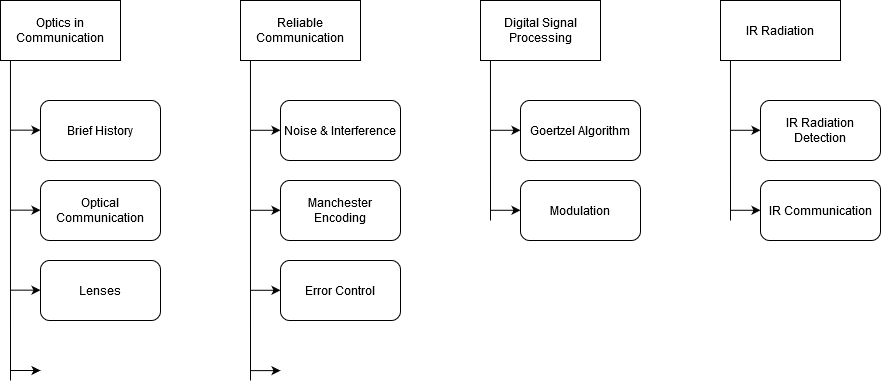
\includegraphics[width=\linewidth]{figures/litreview/litreview_overview.png}
	\caption{Structure of Literature Review}
	\label{fig:litreview_overview}
\end{figure}

%todo: give a structure overview
The review begins with a brief history of optics and the use of optics in digital communication. 

\section{Optics}

\subsection{Brief History}
%The branch of physics that deals with the properties and phenomena of visible light (and by extension other forms of electromagnetic radiation), sometimes esp. concerning sight.

Optics, as defined by the Oxford English Dictionary, is ``The scientific study of sight and the behaviour of light, or the properties of transmission and deflection of other forms of radiation" \cite{oroptics2010}.

For most of human history, little was known of the complex phenomena we call light. The first attempts to understand the properties of light were philosophical and history tells us that the Greek philosophers took interest in the subject. Around 300BC Euclid postulated that light propagated in a rectilinear fashion. He also stated the law of reflection. These principles still form part of our understanding of light today. \cite{Vohnsen2004}

%Well before any established scientific theories existed, lenses have been used as visual aids. Only later in the 17th century can the first record of telescopes be found. Galileo was the first to write about the use of such devices for scientific inquiry.

The use of light for electronic communication only became possible after the advances in semiconductor technologies in the 1960s \cite{Huurdeman2003}. Progress in the development of the light-emitting diode (LED) made it possible to precisely control a light source at very high frequencies, which is necessary to achieve a respectable channel bandwidth.

It did not take long for the infrared LED to be integrated into consumer devices such as the television remote and then later into video cameras as a cost-effective night vision feature. In more recent decades the number of available licenced bands in the electromagnetic spectrum has become increasingly scarce. As a result, there has been a movement to optical wireless communication (OWC), a type of wireless communication that uses visible (and near-visible) light radiation for short-range, high bandwidth communication links.

With the decrease in costs associated with LEDs, transistors and microcontrollers recreational games such as laser tag become possible and the idea was first patented in 1987 \cite{Carter1986}.



\subsection{Lenses}
\label{sec:lit_lenses}
%todo: work on the image presentation format (subfigures)
This project requires the use of a lens to focus a source of light into a narrow beam. Lenses work on the principle of refraction. When light enters a medium with a different refractive index at an angle offset from the perpendicular (normal), the light is bent toward or away from the normal, behaviour described by Snell's law.

When working with lenses, the lens equation may be used to determine how an object might form a real image or virtual image when viewed through a lens \cite{Knight2013}, however for this investigation the definition of the focal length is sufficient.

\begin{figure}[H]
	\centering
	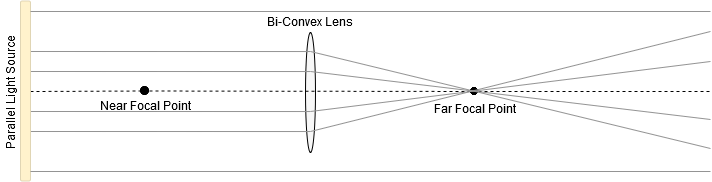
\includegraphics[width=0.8\linewidth]{figures/litreview/lens_diagram.png}
	\caption{Focal Point Illustration}
	\label{fig:lens_diagram}
\end{figure}

Figure \ref{fig:lens_diagram} above shows the near and far focal points for a lens. The diagram illustrates the behaviour of light rays produced by a theoretical parallel light source and passing through a bi-convex lens. The focal point is the common location through which parallel beams of light passing through a convex lens will pass. The near focal point is the point location from which diverging beams would appear to have originated, should the lens in figure \ref{fig:lens_diagram} have been concave.

It is in the interest of this investigation to consider the use of a lens to produce a beam of parallel light rays. This is essentially reversing the process illustrated in figure \ref{fig:lens_diagram}.

\begin{figure}[H]
	\centering
	\begin{minipage}{.3\textwidth}
		\centering
		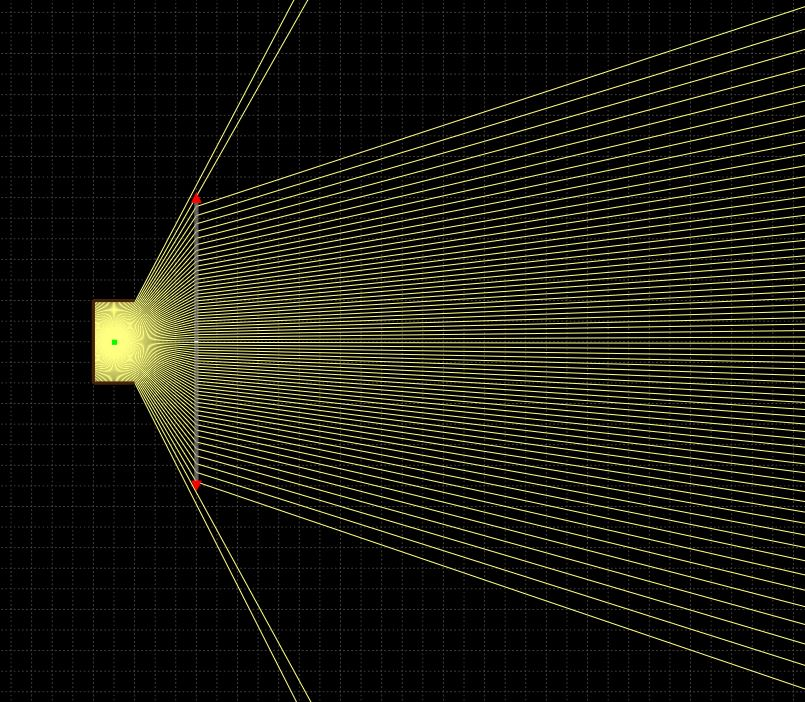
\includegraphics[width=.9\linewidth]{figures/litreview/lens_divergent_beam.JPG}
		\captionof{figure}{Divergent}
		\label{fig:lens_divergent}
	\end{minipage}%
	\begin{minipage}{.3\textwidth}
		\centering
		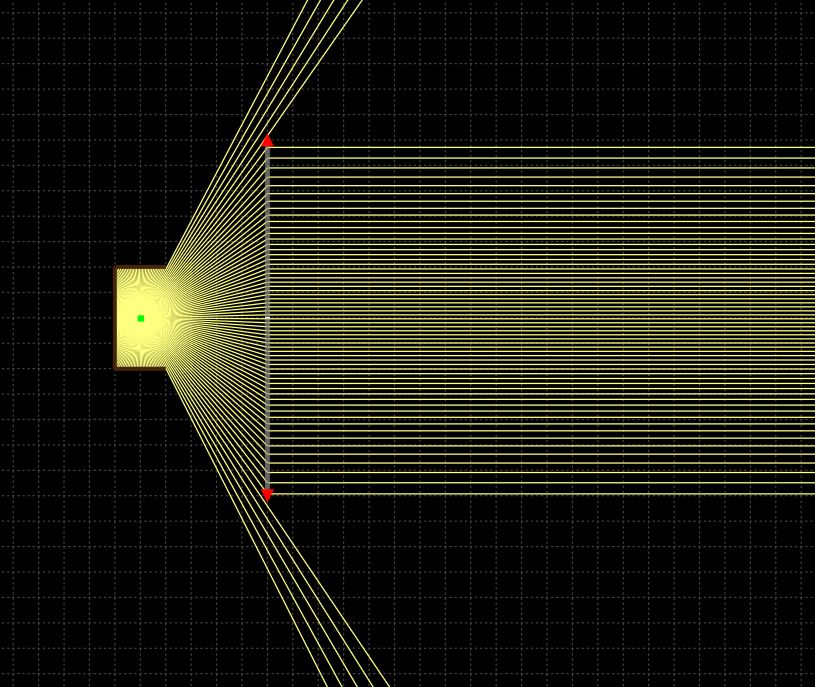
\includegraphics[width=.9\linewidth]{figures/litreview/lens_parallel_beam.JPG}
		\captionof{figure}{Parallel}
		\label{fig:lens_parallel}
	\end{minipage}
	\begin{minipage}{.3\textwidth}
		\centering
		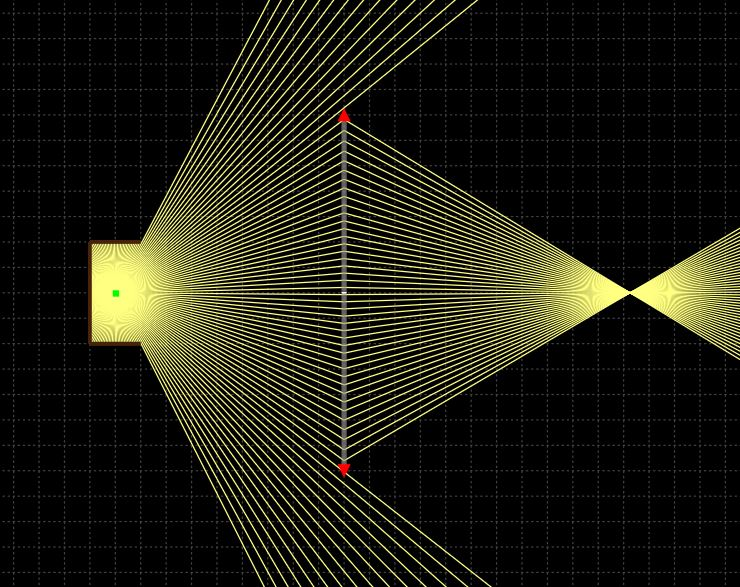
\includegraphics[width=.9\linewidth]{figures/litreview/lens_focus_beam.JPG}
		\captionof{figure}{Convergent}
		\label{fig:lens_convergent}
	\end{minipage}
	\caption*{Images showing the different behaviours of light interacting with a lens\footnotemark}
\end{figure}

\footnotetext{Created using \href{https://ricktu288.github.io/ray-optics/simulator/}{Ray-Optics Simulator}}

Figures \ref{fig:lens_divergent} to \ref{fig:lens_convergent} illustrate the three behaviours that may be achieved using a single point source of light and an ideal lens. Light diverges after passing through a lens as shown in figure \ref{fig:lens_divergent} when a point light source exists between the near focal point and the lens. Figure \ref{fig:lens_parallel} shows that for a point light source placed at the focal point, parallel rays of light will emerge from the lens. It should be noted that the parallel rays produced in this manner form a beam with a diameter the same size as the lens. Finally, figure \ref{fig:lens_convergent} illustrates that placing a point light source beyond the near focal point (on the opposite side to the lens) results in a beam that initially converges, focusing to some point and then diverges.

\subsection{Optical Sensing}
\label{sec:optical_sensing}

\subsubsection{Optical Detectors}
In his paper on optical detectors, Forrest highlights the three main contenders for converting light to an electrical signal. These are the PIN diode, avalanche photodiode and photoconductor \cite{Forrest1986}.

\textbf{Photoconductor}\\
The photoconductor is an optical sensor constructed from intrinsic semiconductor material. This un-doped material changes resistance in proportion to incident light of a particular wavelength. Unlike extrinsic semiconductor devices, no current is induced in a photoconductor as the photoelectric effect does not apply. Properties such as the sensitivity to different wavelengths of light depend solely on the semiconducting material of the photoconductor \cite{Kingston2003}.

\textbf{PIN Photodiode}\\
The PIN diode is constructed out of semiconductor material with two doped regions. As the name implies PIN diodes are constructed by separating a positively doped (P-region) and negatively doped (N-region) with an intrinsic region.

\begin{figure}[H]
	\centering
	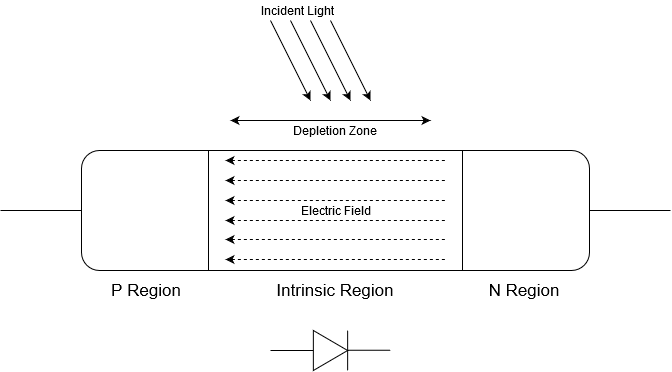
\includegraphics[width=0.8\linewidth]{figures/litreview/pin_diode_diagram.png}
	\caption{PIN Diode Construction and Operation as an Optical Sensor}
	\label{fig:pin_diode_diagram}
\end{figure}

Figure \ref{fig:pin_diode_diagram} above illustrates the working principle of the PIN photodiode.
When photons with a high enough energy are absorbed by the depletion region of the diode, an electron is freed. This free electron accelerates due to the electric field which induces a current.

Typically the diode is reverse biased to increase the strength of the electric field between the two doped regions. Under reverse bias conditions, a small current flows independent of whether light is shone on the depletion zone, this current is known as dark current.

\textbf{Avalanche Photodiode}\\
The avalanche photodiode is a modification to the structure of the PIN diode. In the case of the avalanche photodiode, an additional P-region is placed adjacent to the N-region. This additional P-region forms the avalanche region. The avalanche photodiode can be made sensitive enough to allow the detection of individual photons \cite{Perenzoni2018}.

\textbf{Phototransistor}\\
The phototransistor is another component capable of detecting light. The construction of a phototransistor is similar to that of a regular transistor, but rather than use an electrical signal to control the base current, a photodiode is used.

Phototransistors allow a much larger amount of current to flow for the same amount of light when compared to regular photodiodes.

\subsubsection{Amplification}

Circuits which convert small current into voltages are known as trans-impedance amplifiers (TIA). They are used in applications where the current response through the device is much more linear than the voltage.

\begin{figure}[H]
	\centering
	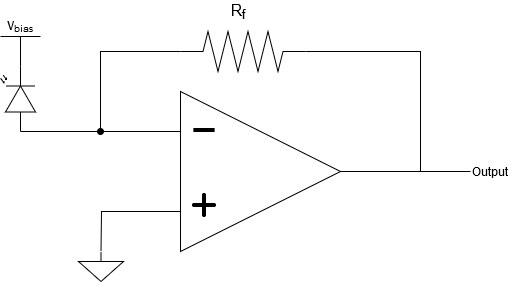
\includegraphics[width=0.6\linewidth]{figures/litreview/transimpedance_amplifier.png}
	\caption{Fundamental Trans-impedance Amplifier}
	\label{fig:transimpedance_amplifier}
\end{figure}

The most simple design comprises an operational amplifier with a single feedback resistor as illustrated in figure \ref{fig:transimpedance_amplifier}.

Many variations of this design exist, each built to achieve different levels of performance, for example in their paper on developing a lock-in amplifier for optical sensors, Ferreira and Petraglia use a constant current source rather than a fixed reverse bias voltage to minimize the shot noise caused by dark current \cite{Ferreira2017}.


%%%%%%%%%%%%%%%%%%


\section{Optical Communication}
Optical communication concerns all manors of communicating information from one party to another through the medium of light. This investigation focuses on the use of light as a means of communication between electronic systems.

\subsection{Optical Communication Techniques} %todo: better name for this 'catergories of techniques' 

Most light-based communication methods may be classified as \textit{free-space optical communication} techniques. These techniques do not require any physical medium between the receiver and transmitter. Not all light-based communication is performed in free space, for example, fibre optic communication which is among the fastest-growing optical communication techniques of recent times.

Fibre optic communication uses a physical cable designed to guide a beam of light using the principles of total internal reflection. Fibre-optic communication systems may utilize an LED or laser diode to produce an optically encoded digital signal. Recent developments in vertical-cavity surface-emitting lasers (VCSEL) have resulted in more fibre optic systems turning to this technology.

Free-space optical communication uses much the same technology to transmit information through light, however, in the field of optical wireless communications the technology is integrated into regular lighting solutions. The result is %todo: fix this paragraph - its too much waffle



\subsection{IR Communication}
%This is where I talk about different IR protocols

IR has is used in many applications, this is because it is cheap, efficient and simple to use. A basic implementation might consist only of an IR LED, IR receiver IC and a pair of microcontrollers. The most commonly used band of IR radiation for communication is between 780nm and 950nm, this is as a result of the availability of low-cost LEDs and quality photodiodes that operate in this frequency band \cite{Elgala2011}.

Many modulation techniques have been developed for optical wireless communication. These range from advanced techniques such as multiple-subcarrier modulation (MSM) to basic techniques such as on-off keying (OOK) and pulse position modulation (PPM).

Multiple-subcarrier modulation sums numerous sub-carrier signals and uses the result to modulate the light source. As a consequence of using multiple low-frequency sub-carriers, it is possible to achieve a high total bit rate with little distortion, removing the need for equalization \cite{Ohtsuki2003}.

Notable tradeoffs for techniques that increase the bit-rate are diminishing range, lower resistance to ambient noise and an increase in system complexity. To communicate between a tagger and target in laser tag, high bandwidth is not required. It is therefore advantageous to utilize a more robust technique with a lower bit-rate such as on-off keying.

OOK is utilized in many systems, for example, in remote control applications. As a result, there are several IR communication protocols based on this technique. The following are a few of the popular options

\begin{itemize}
	\item RC-5
	\item RC-6
	\item NEC
	\item SIRC
\end{itemize}

Each of these protocols is based on OOK, but differ in how they define symbols. To represent two different states, an IR source is modulated at a chosen carrier frequency (usually around 36kHz). When the light source is modulating the signal is \textit{on} and when the source is not modulating the signal is \textit{off}.  Modulation makes it possible to distinguish between a generated IR signal and ambient IR radiation from noise sources.

Protocols such as Sony's SIRC use a technique known as pulse width encoding. This technique involves modulating the IR LED for a different period depending on whether a 1 or 0 is to be transmitted while maintaining a constant time between transmissions.

Protocols such as the NEC protocol by Renesas use pulse distance encoding. This protocol specifies a different off period between on pulses to distinguish between a logical 1 and 0.

The RC-5 protocol and its successor the RC-6 protocol use Manchester Encoding to transfer binary information. Due to its wide adoption and popularity \cite{rudrappa2009}, an adaption the RC-5 protocol will be used in this project. Manchester Encoding is reviewed in section \ref{sec:manchester_encoding} below.

\subsubsection{RC-5 Protocol}
\label{sec:rc_5_protocol}
The the RC-5 protocol is illustrated in figure \ref{fig:rc_5_protocol}. The bits are encoded using the IEEE 802.3 convention for Manchester Encoding. The modulation frequency of the carrier is 36kHz and the length of one bit period is 64 cycles or 1.778mS\cite{Perme2007}.

\begin{figure}[H]
	\centering
	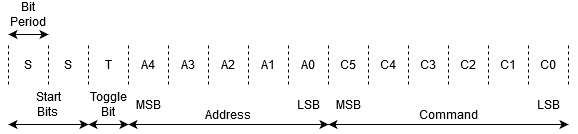
\includegraphics[width=0.8\linewidth]{figures/litreview/rc5_protocol.png}
	\caption{RC-5 IR Protocol}
	\label{fig:rc_5_protocol}
\end{figure}

Every transmission begins with two start bits, these bits always have a value of 1. Following the two start bits is the `toggle' bit. In remote control applications, it is useful to distinguish between a button which remains depressed and a button being repeatedly pressed. This is achieved through the toggle bit which is flipped each time a button is released. When a button remains depressed, the message is transmitted repeatedly with a 114ms gap between transmissions. Finally, the RC-5 protocol data is structured such that it first transmits a 5-bit address followed by a 6-bit command.


%\subsection{Materials Interaction}
%Talk briefly about materials and the interaction of different materials with IR. Mention the difficulty of acquiring these resources and therefore the exclusion of them during experimentation


\subsection{Communication System Structure} 

In the book \textit{Principles of LED Light Communications}, Dimitrov and Harald present the generalized system setup for an optical wireless communication system. Figure \ref{fig:system_configuartion_lit} below is a recreation of the system building blocks diagram shown on page 14 \cite{Dimitrov2015}.

\begin{figure}[H]
	\centering
	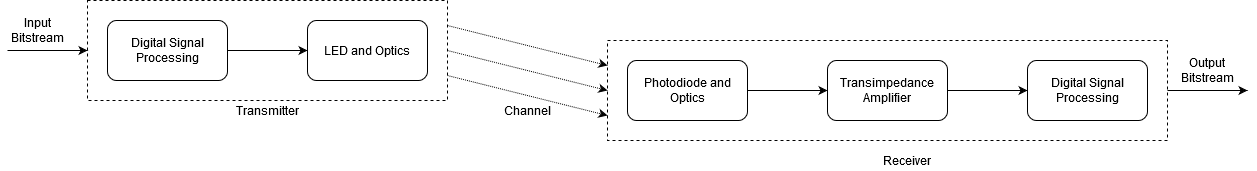
\includegraphics[width=\linewidth]{figures/litreview/system_configuartion_lit.png}
	\caption{Communication System Setup}
	\label{fig:system_configuartion_lit}
\end{figure}

The digital signal processing stage of the transmitter is responsible for encoding the incoming bitstream and generating the analog modulating signal. The LED and optics stage is responsible for amplifying this analog signal and generating light output.

The channel is the optical free-space path through which the light reaches the receiver. This path depends on the directionality of the receiver and transmitter and the relative orientation of the two systems. In the context of laser tag, the transmitter optics are highly directional while the receiver optics, in the ideal case, are omnidirectional. Because of the directionality of the transmitter, this is referred to as a line of sight (LOS) link configuration.

It should be noted that an anti-alias filtering stage is implicit in the path between the output of transimpedance amplifier and the input to the digital signal processing stage of the receiver.


%%%%%%%%%%%%%%%%%%

\section{Reliable Data Transmission}

\subsection{Noise \& Interference}
%Talk about modulation (and demodulation) techniques 
% no seperate \subsection{Demodulation}
%Give an overview of demodulating and what techniques exist: Goertzel, DFT, tone-detectors, next sections highlights details

%%Make this into a sub-sub section and include it under modulation
%\subsubsection{}
%Talk about interference and noise, sources and narrow down to IR in particular... Also, note noise in components and power supplies etc.

Optical wireless communication is susceptible to interference and noise produced by most sources of light because it operates on the same band of frequencies as visible light. Light sources such as incandescent light bulbs and the sun produce white noise in the infrared region, while modulated light sources such as the fluorescent light produce cyclostationary noise \cite{Carruther2000}.

To overcome noise and various forms of interference, digital modulation is commonly used. There are several modulation techniques based on keying, these are tabulated in table \ref{tbl:types_of_keying}. In keying, a finite set of states are defined and the output waveform transitions between these predefined states during modulation.

\begin{table}[H]
	\centering
	\begin{tabular}{cc}
		\hline
		\textbf{Modulation Technique} & \textbf{Description} \\ \hline
		Phase-Shift Keying & Finite set of phase shifts \\ \hline
		Frequency-Shift Keying & Finite set of tones \\ \hline
		Amplitude-Shift Keying & Finite set of amplitudes \\ \hline
	\end{tabular}
	\caption{Digital Modulation - Fundamental Techniques}
	\label{tbl:types_of_keying}
\end{table}


In addition to noise and interference, saturation can also disrupt a transmission. Saturation occurs when the incident light on the detector is of such a high intensity that any changes in light amplitude go undetected. To reduce the likelihood of saturation, filters are placed over the sensor to allow only light of a specific wavelength to reach the sensor.



\subsection{Manchester Encoding}
\label{sec:manchester_encoding}
Manchester Code is a type of phase encoding. It is classified as a line code and is produced by generating patterns through some measurable phenomena. The commonly used mediums to represent a Manchester encoded signal would be voltage, current and light (electromagnetic radiation).

Manchester coding, as its name suggests, was developed at the University of Manchester and it was first published in 1949 \cite{Jameel2019}. Manchester encoding is a protocol for integrating the clock and data into a single sequence consisting of only two symbols. It does not require clock synchronization, only that a predefined bit-width is known by both the receiver and transmitter. 

The principle behind Manchester code is to encode the information into transitions between two symbols. This technique makes the encoding scheme particularly useful in communication employing inductive coupling such as in RFID. Due to its self-clocking property and simplicity, it is the standard means of encoding for many IR applications. Perhaps the most common application is in the remote controls we use for various appliances.

Manchester code is a special form of binary phase-shift keying (BPSK). A square wave of a particular frequency is chosen as the carrier and binary information is encoding by adjusting the setting a phase offset to either 0\degree or 180\degree s. In figure \ref{fig:manchesterencoding} the process of encoding 10 bits is illustrated. Two conventions exist, their difference lies solely in the definition of which logic values are represented by each of the two transitions. The convention used throughout this investigation is per the IEEE 802.3 standard which defines a logical one as the transition from 0 to 1 and a logical zero as 1 to 0. The other convention used by inventor G.E. Thomas is the inverse of this and is also widely used.\\

\begin{figure}[H]
	\centering
	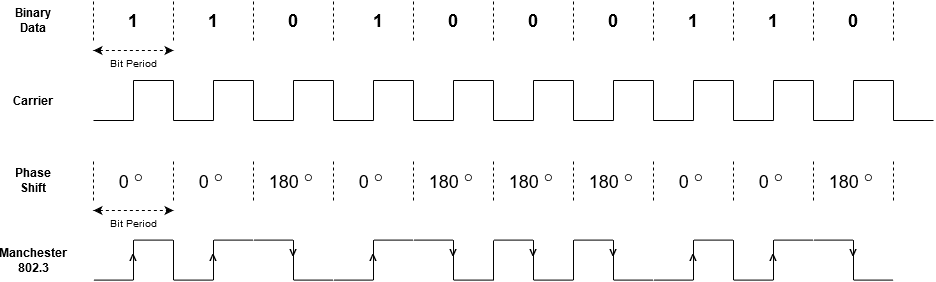
\includegraphics[width=0.7\linewidth]{figures/litreview/manchester_encoding}
	\caption{Manchester code example using 10 bits}
	\label{fig:manchesterencoding}
\end{figure}

\subsubsection{Encoding Algorithm}

Using a timer to toggle a boolean 180\textdegree{} out of phase with the carrier frequency, it is possible to determine the current output state of the Manchester waveform using the XOR operation as shown in equation \ref{eqn:manchesterencode}.

\begin{equation}
	\label{eqn:manchesterencode}
	manchester\_out = bit\_period \oplus tx\_bit
\end{equation}

$bit\_period$ is 180\textdegree{} out of phase with the carrier waveform. $tx\_bit$ is the binary value being encoded and $manchester\_out$ is the logical value of the Manchester output waveform.


\subsubsection{Decoding Algorithm}
Different techniques have been developed to decode Manchester encoded sequences. In his paper on methods for decoding Manchester code, R. A. Dobre discusses an elegant and widely used finite state machine approach which has been illustrated in figure \ref{fig:manchesterdecodingfsm} below. \cite{Dobre2014}

\begin{figure}[H]
	\centering
	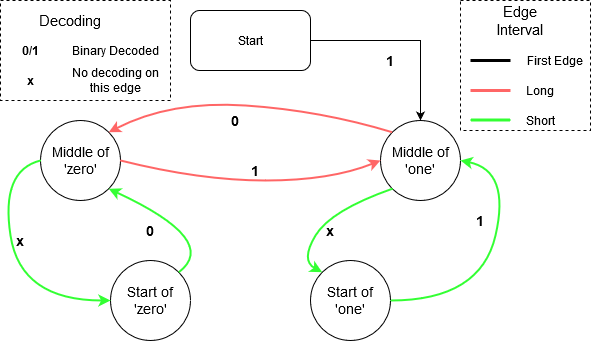
\includegraphics[width=0.7\linewidth]{figures/litreview/manchester_decoding_fsm.png}
	\caption{FSM Algorithm for Decoding Manchester Sequences}
	\label{fig:manchesterdecodingfsm}
\end{figure}

The state machine approach is particularly useful because it only considers the period between the detected edge and the previous edge. It removes the need to track samples saving on memory and reducing processing power requirements, all without introducing additional complexity.

It should be noted that this FSM assumes the first bit transmitted is always a logical 1. It also does not detect the end of a sequence, so additional logic is required to detect when a certain number of bits have been received or to implement a timeout timer.

%\iffalse
\subsection{Error Control}

In information theory, error control is the field of study that concerns detecting errors in digital communications and the techniques used to correct those errors. Whenever data is transmitted over some kind of network, there is the possibility that interference can cause a bit to flip resulting in an error. Richard Hamming pioneered in the development of digital error control and is known for (amongst other things) the Hamming code.

Various ways to detect and potentially correct the presence of an error. The most trivial technique known as a 'repetition code' simply involves sending the information three times, making it possible to detect if one of the three data-streams doesn't match the others. Although repetition codes allow for both error detection and correction, it is extremely inefficient. Various techniques have been developed and each technique balances complexity and efficiency.

\subsubsection{Parity}
Using a parity bit is possibly the most simple method to detect an error in a bit sequence. The parity of a sequence may be defined as the result of a bitwise exclusive or (XOR) operation, this is known as 'even parity' because the parity bit value is chosen such that upon appending it to the bit-sequence there would be an even number of 1s. Conversely 'odd parity' calculates the parity bit such the number of 1s in the generated sequence is odd. Table \ref{tbl:party_examples} below provides example bit sequences and the respective even (given by the XOR operation) and odd parity values.

\begin{table}[H]
	\centering
	\begin{tabular}{ccc}
		\hline
		\multicolumn{1}{l}{\textbf{Bit Sequence}} & \textbf{XOR of Bits} & \multicolumn{1}{l}{\textbf{Odd Parity Bit}} \\ \hline
		0000000 & 0 & 1 \\ \hline
		1111111 & 1 & 0 \\ \hline
		1010101 & 0 & 1 \\ \hline
		1001100 & 1 & 0 \\ \hline
	\end{tabular}
	\caption{Even and odd parity for example bit sequences}
	\label{tbl:party_examples}
\end{table}

To use parity as a method to detect errors, the sender and receiver choose to use either even or odd parity. Before transmission, the sender calculates the parity bit for the sequence to be sent, this bit is then appended to the bit-stream. Upon receiving the bit-stream, the same parity calculation is done on the sequence. If the result of this calculation is a 1 it can be said for certain that an error occurred, if the result is zero it can be said that no error occurred or an even number of errors occurred.

%decided to exclude
%\subsubsection{Hamming Code}
%talk briefly on Hamming Codes (and why it was excluded)





%%%%%%%%%%%%%%%%%%
\section{Digital Signal Processing}
In the age of microcontrollers and microprocessors, in many situations, it has become far more effective to use digital signal processing to manipulate and processes signals.

Part of the IR decoding process requires detecting the presence of a particular frequency (commonly referred to as a tone). The natural tool to turn to when examining the frequency content of a signal is the discrete Fourier transform (DFT). The DFT is well established and there exist a variety of algorithms which compute its values, perhaps the most well known being the FFT. However, to detect a single tone of a predetermined frequency, the DFT is not the most efficient method, even when optimized algorithms such as the FFT are implemented.

The FFT provides a very efficient means for determining all the DFT coefficients, but in a use case only a few of the coefficients are used and the rest discarded it is not the most efficient technique. By using a less efficient process for calculating individual coefficients of the DFT it is possible to greatly reduce program complexity and processing time relative to an implementation that uses the FFT.


\subsubsection{Analog Preprocessing}

Any time an analog signal is sampled for digital signal processing, it must be filtered to remove any frequencies above the Nyquist frequency. The Nyquist frequency is defined in equation \ref{eqn:nyquist}. If frequencies higher than the Nyquist frequency are present in the sampled waveform, aliasing will occur. Naturally, this filtering stage cannot be performed digitally and therefore an analog filter must be implemented.

%%%%%%%%%%%%%
\begin{equation}
	f_{Nyquist} = \frac{f_{sampling}}{2}
	\label{eqn:nyquist}
\end{equation}

%%%%%%%%%%%%%

In addition to filtering, it is sometimes necessary to perform other operations on analog signals before they are sampled, such as rectification or adding a positive offset to ensure the signal is within the input range of the ADC.

\textbf{Low Pass Filtering}\\
Anti-alias filters are built to suppress high frequencies, many different approaches to filtering high frequencies exist. The most basic filter is a passive RC network as shown in figure \ref{fig:filter_basic_lpf}. Filters with a sharper cut-off can be created by using an operational amplifier, figure \ref{fig:vcvs_filter_lpf} shows a voltage-controlled voltage source (VCVS) circuit configured as a 2nd order low pass filter. The circuit in figure \ref{fig:vcvs_filter_lpf} can be found in the book \textit{The art of electronics - 2nd Edition} on page 274, also included in this book is a table of coefficients which may be used to achieve the desired filter response \cite{Horowitz1995}. Finally, IC's containing customizable second-order filtering stages can be purchased such as the \href{https://www.maximintegrated.com/en/products/analog/analog-filters/MAX275.html/tb_tab0}{MAX275} series by maximum integrated.

\begin{figure}[H]
	\centering
	\begin{minipage}{.42\textwidth}
		\centering
		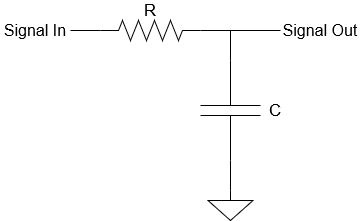
\includegraphics[width=.9\linewidth]{figures/litreview/filter_basic.png}
		\captionof{figure}{Simple RC Network - LPF Configuration}
		\label{fig:filter_basic_lpf}
	\end{minipage}%
	\hfill
	\begin{minipage}{.54\textwidth}
		\centering
		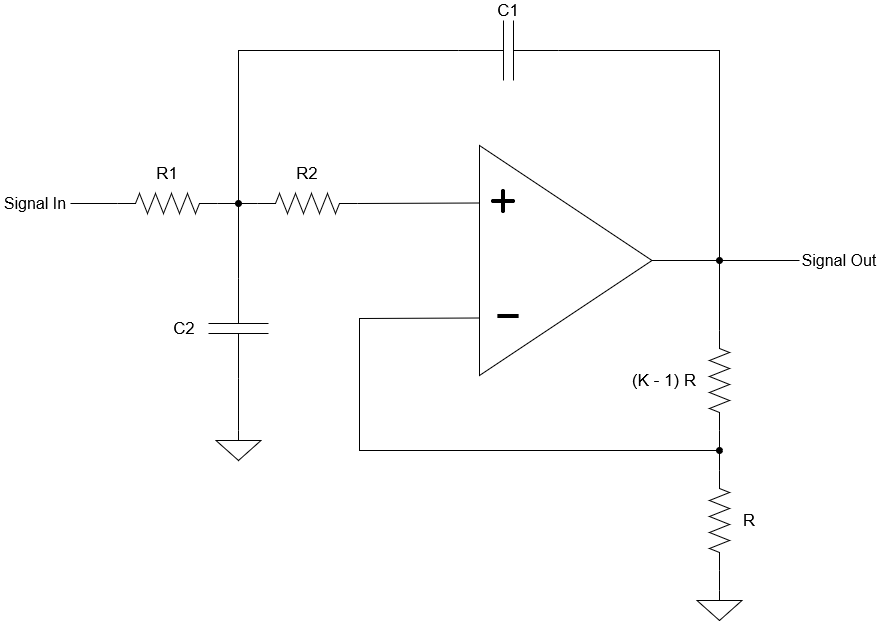
\includegraphics[width=.9\linewidth]{figures/litreview/vcvs_filter.png}
		\captionof{figure}{Voltage Controlled Voltage Source - LPF Configuration}
		\label{fig:vcvs_filter_lpf}
	\end{minipage}
\end{figure}

Dedicated filtering IC's are useful in precision applications where reproducibility and consistency of filter performance is a priority. They also allow for the construction of digitally controllable analog filters \cite{Huijing2010}. Dedicated filtering IC's are comparably expensive and therefore a trade-off between cost and convenience must be considered.

\textbf{Precision Rectification}\\
Simple, half-wave rectification may be achieved simply by placing a diode in series with the path of a signal. However, due to the forward voltage drop of the diode, any positive portion of the waveform below the forward voltage of the diode will be lost. This non-ideal effect can be mitigated through the use of an operational amplifier.

\begin{figure}[H]
	\centering
	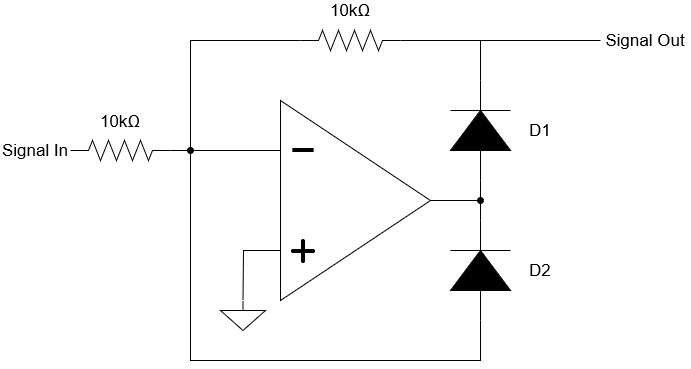
\includegraphics[width=0.6\linewidth]{figures/litreview/precision_rectifier.png}
	\caption{Precision Rectifier}
	\label{fig:precision_rectifier}
\end{figure}

There are various circuit designs which use an operational amplifier to mitigate the effect of the diode forward voltage drop, they are known as precision rectifiers. The circuit in figure \ref{fig:precision_rectifier} is one of the more sophisticated designs as the output of the op-amp has a maximum swing of two diode drops. In simpler designs, the operational amplifier might swing more than half the supply rails during operation. The design has been taken from \textit{The art of electronics - 2nd Edition} and may be found on page 188 \cite{Horowitz1995}.



\subsection{Goertzel Algorithm}
\label{sec:goertzel_lit_review}

The algorithm which computes individual DFT coefficients is known as the Goertzel algorithm (or Goertzel Filter) and was developed by G. Goertzel in 1958. \cite{Goertzel1958} A common application of the Goertzel algorithm is in the decoding of DTMF\footnotemark{} signals.
\footnotetext{Dual Tone Multiple Frequency}

\subsubsection{Derivation}
The Goertzel algorithm may be derived from the formula for the DFT. In the derivation \(W_N = e^{-j\frac{2\pi}{N}}\).

\begin{equation}
\label{eqn:dft_defn}
X[k] = \sum_{n=0}^{N-1}x[n]W_{N}^{nk}
\end{equation}

Multipling the right side of equation \ref{eqn:dft_defn} by \(W_{N}^{-Nk} = e^{j\frac{2\pi N k}{N}} = 1\) we get

\begin{equation}
X[k] = W_{N}^{-Nk}\sum_{n=0}^{N-1}x[n]W_{N}^{nk}
\end{equation}

Rearranging we get

\begin{equation}
\label{eqn:dft_conv}
X[k] = \sum_{n=0}^{N-1}x[n]W_{N}^{k(n-N)}
\end{equation}

Notice that if we consider the signal \(h_k[l] = W_N^{-kl}u[l]\), then equation \ref{eqn:dft_conv} is the convolution of $h_k[l]$ with $x[l]$. Substituting these signals into equation \ref{eqn:dconv} (formula for discrete convolution) below, we can rearrange the result to arrive at equation \ref{eqn:dconv_sub}.

\begin{equation}
\label{eqn:dconv}
y_k[l] = \sum_{m=0}^{N-1}x[m]h_k[l - m]
\end{equation}

\begin{equation}
\label{eqn:dconv_sub}
y_k[l] = \sum_{m=0}^{N-1}x[m]W_N^{k(m-l)}
\end{equation}

Comparing equation \ref{eqn:dft_conv} with equation \ref{eqn:dconv_sub}, it becomes clear that from the convolution $y_k[n] = x[n] * h_k[n]$ we can find the value of $X[k]$ by substituding N into $y_k[n]$. Thus the following relationship exists

\begin{equation}
\label{eqn:goertzel_relationship}
X[k] = y_k[N]
\end{equation}

%%%%
%Now deriving the filter
%%%%

In their paper on generalizing the Goertzel algorithm for non-integer multiples of the fundamental frequency, P. Sysel and P. Rajmic show how the function $h_k[n]$ may be transformed to the Z-domain and optimized to reduce the amount of computational power required to compute the DFT coefficient \cite{Sysel2012}. The results are given by the following equations.

%The following equations are taken from the paper - check if that's okay with Simon...
\[h_k[n] \xRightarrow{\text{Z}} H_k(z)\]

\begin{equation}
W_N^{-kl}u[n] \xRightarrow{\text{Z}} \frac{1}{1 - W_N^{-k}z^{-1}} = \frac{1}{1 - e^{j\frac{2\pi k}{N}}z^{-1}}
\end{equation}

$H_k(z)$ can then be manipulated to give

\begin{equation}
\label{eqn:g_optimized_ir}
H_k(z) = \frac{1 - e^{-j\frac{2\pi k}{N}}z^{-1}}{1 - 2cos(\frac{2\pi k}{N})z^{-1} + z^{-2}}
\end{equation}

Finally, equation \ref{eqn:g_optimized_ir} can be converted to state variable form to yield the following


\begin{equation}
\label{eqn:g_ss}
s[n] = x[n]+2cos(\frac{2\pi k}{N})s[n-1]-s[n-2]
\end{equation}


\begin{equation}
\label{eqn:g_ssoutput}
y_k[n] = s[n]-e^{-j\frac{2\pi k}{N}}s[n-1]
\end{equation}



\subsubsection{Implementation}
\label{sec:goertzel_implementation}
Using the state variable equations \ref{eqn:g_ss} and \ref{eqn:g_ssoutput} we can implement the goertzel filter digitally. The following code in listing \ref{lst:goertzel_algorithm} shows a Goertzel filter implemented in the Octave environment.

\begin{lstlisting}[caption={Goertzel Algorithm - Octave Implementation\label{lst:goertzel_algorithm}}]
function magnitudesqd = calculate_goertzel (N, bin_frequency, sampling_frequency, samples)

k = round(N*bin_frequency/sampling_frequency);
omega = (2*pi*k)/N;
cosval = cos(omega);
sinval = sin(omega);
coeff = 2*cosval;

s1 = 0;
s2 = 0;

for i = 1:N
s0 = (samples(i) + (coeff*s1) - s2);
s2 = s1;
s1 = s0;    
end

realv = (s1 - (s2 * cosval));
imgv = (s2 * sinval);  

magnitudesqd = realv*realv + imgv*imgv;

endfunction
\end{lstlisting}

%%%%%%%%%%%%%%%%%%








